\section{System Overview of REMARK} \label{sec:system}
%
To address the two challenges raised in Sec.~\ref{sec:motivation}, this paper proposes REMARK, an efficient and reliable multi-device checkpointing framework.
Fig.~\ref{fig:SystemArchitecture} shows the overview of REMARK framework, which contains an enhanced NVP architecture (Sec.~\ref{sec:hardware}), an offline program transformer (Sec.~\ref{sec:offline}) and an online recover procedure (Sec.~\ref{sec:online}).
The offline transformer pre-sets checkpoints to convert the original program to recoverable program for online execution.
The online recover procedure will adjust the checkpoints dynamically for further efficiency.
%And the hardware architecture provides efficient and flexible processor and peripheral checkpointing function interface.
The rest of this section presents the overview of each component.
The details will be covered in the rest of this paper. 

%\vspace{5pt}
% hardware
\noindent\textbf{Enhanced NVP Hardware Support.} \\
As shown in Fig. 4, on top of existing NVP and NVIO that can instantly backup and restore the system state, REMARK adds four new modules to satisfy the requirements for flexible B/R functions and efficient peripheral recovery in the multi-device checkpointing strategy.

Two of these modules are used to help implement flexible and reliable processor checkpointing.
\textbf{B/R Manager} is designed based on the traditional B/R controller enabling both active and passive B/R operation.
Moreover, bootstrap is also added in this module to control the processor starting procedure.
\textbf{INT Recognizer (IRec)} is used to place safe checkpoint when power failure crashes a hardware interrupt where interactions between processor and peripherals locates.
The other two modules are used to realize efficient peripheral configuration and restart.
\textbf{Peripheral State Registers (PSRs)} is a real-time monitor of the peripheral state to support the efficient selective peripheral configuration.
\textbf{Peripheral Restart Module (PRM)} accelerates the peripheral restart procedure by automatically locating the start function in the program and correctly returning.
With the help of PRM, extra rollback of processor is removed.
To access these new modules, five new instructions are proposed as shown in Table~\ref{tab:InstrSet}.
Design details of the hardware architecture are presented in Sec.~\ref{sec:hardware} and Fig.~\ref{fig:HardwareArchitecture}.


\begin{figure*}[!htbp]
    \centering
    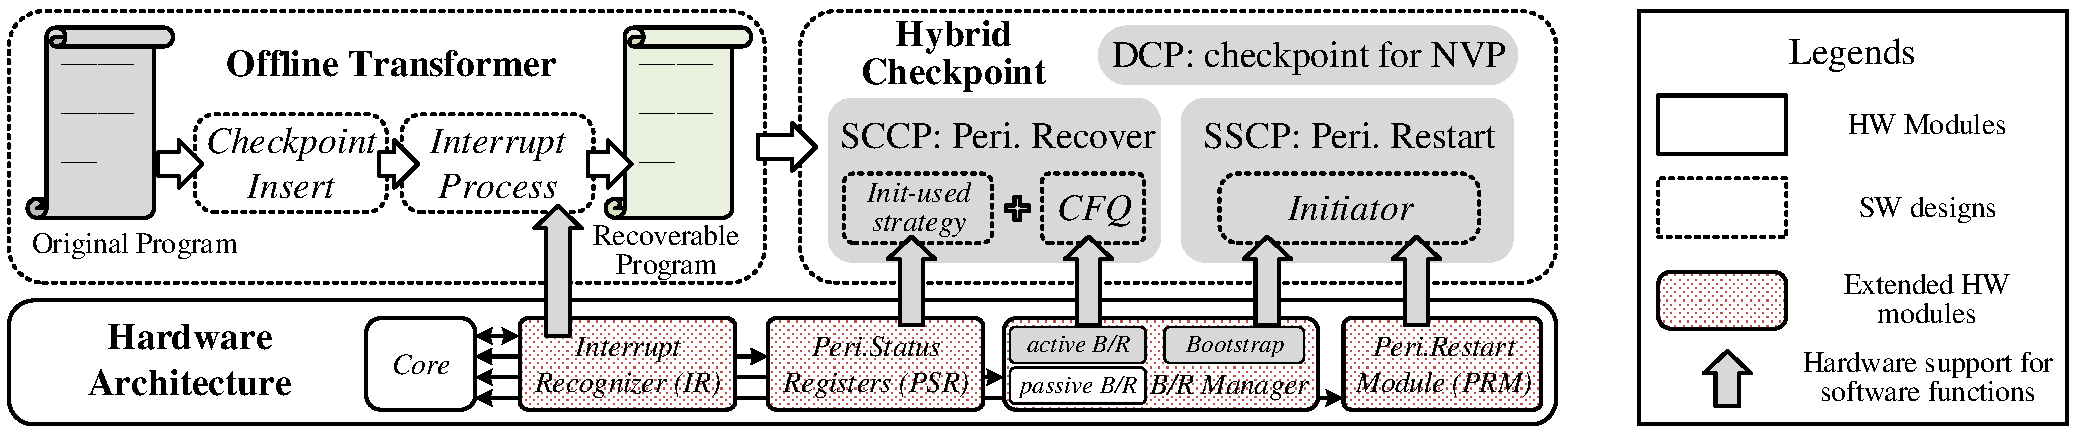
\includegraphics[width=1\textwidth]{Fig3_System.pdf}
    \caption{The HW/SW co-designed system diagram of REMARK.}
    \label{fig:SystemArchitecture}
\end{figure*}

%
\begin{figure*}[!htpb]
    \centering
    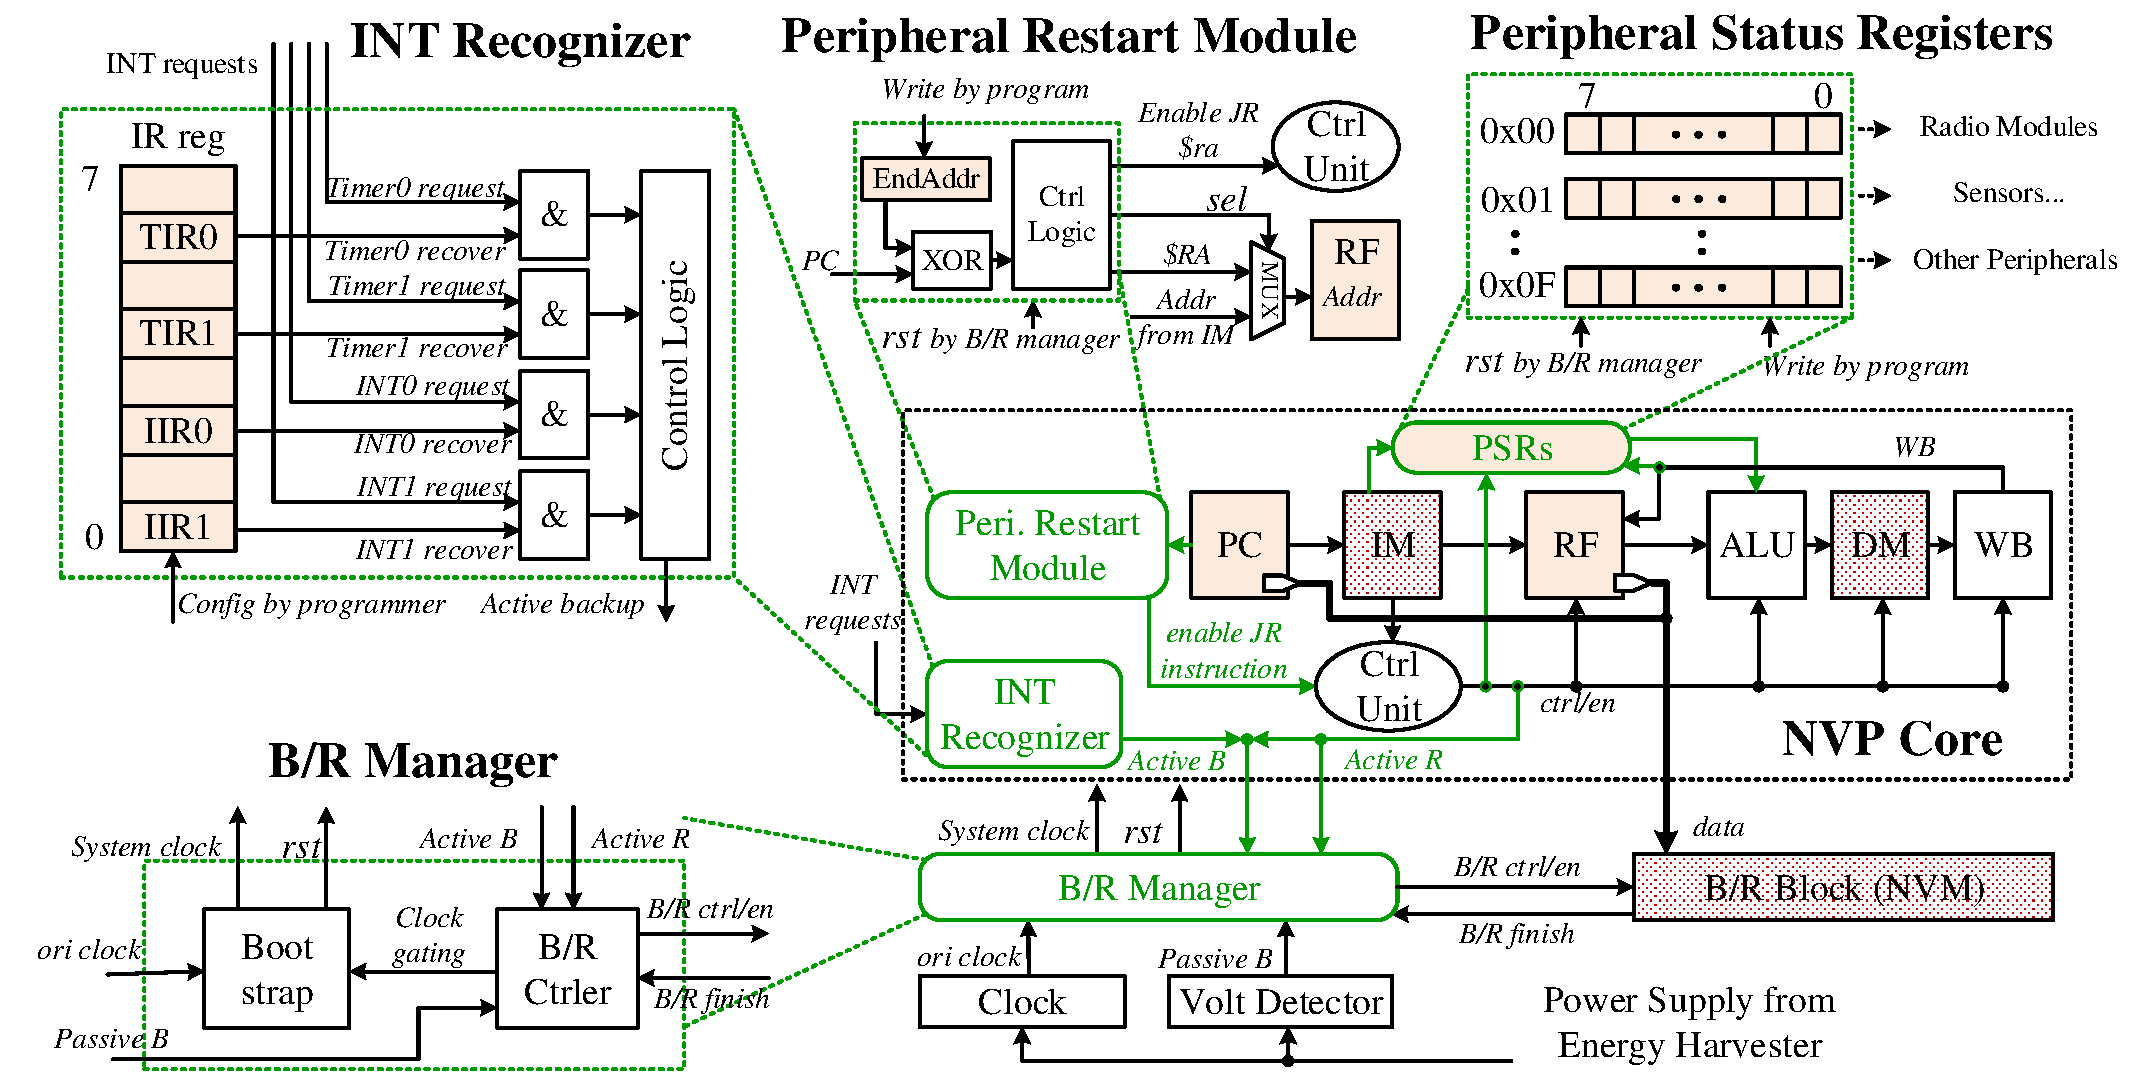
\includegraphics[width=1\textwidth]{Fig4_HardwareArchitecture.pdf}
    \caption{The hardware architecture of REMARK and its main modules. }
    \label{fig:HardwareArchitecture}
\end{figure*}

\begin{figure*}[!htbp]
    \centering
    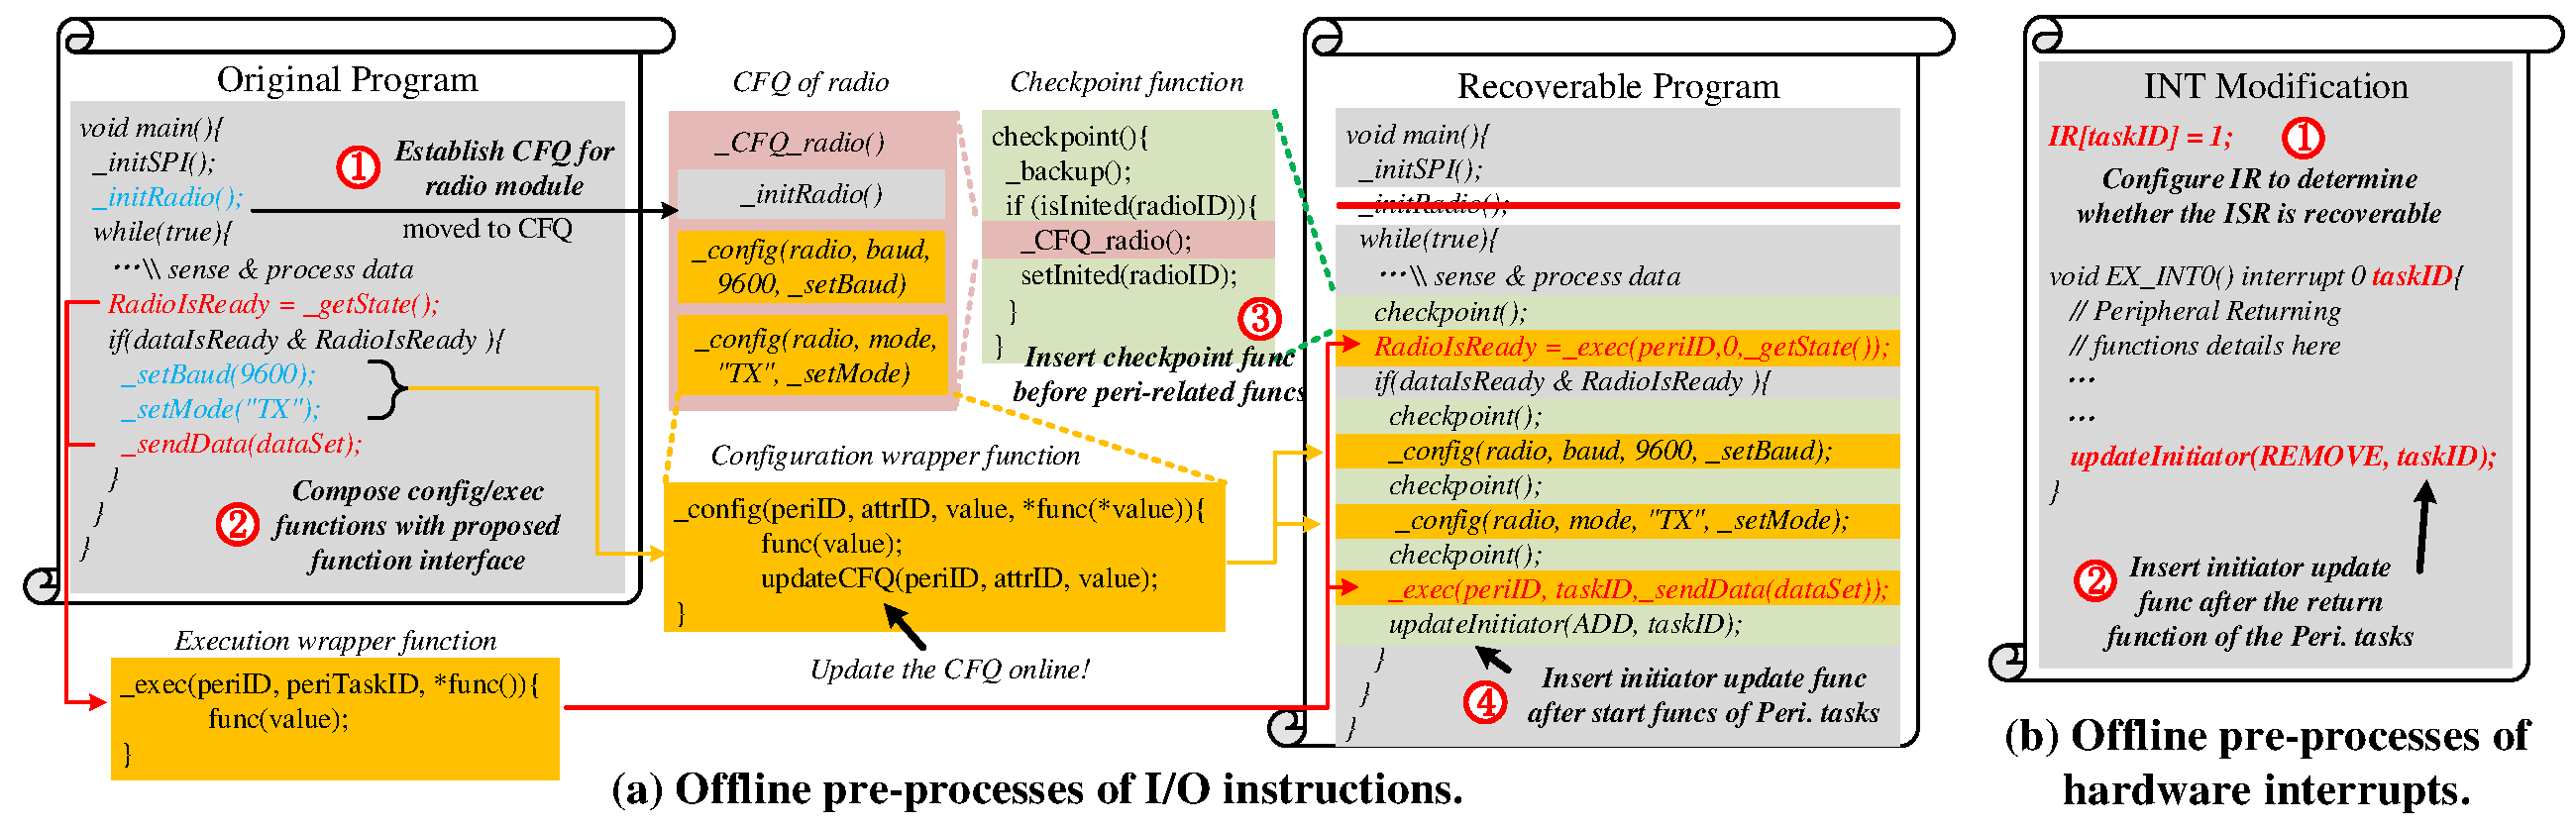
\includegraphics[width=1\textwidth]{Fig5_OfflineStage.pdf}
    \caption{The program pre-processes during the software transformation stage.}
    \label{fig:OfflineStage}
\end{figure*}

% offline
%\vspace{5pt}
\noindent\textbf{Offline Program Transformer.} \\
REMARK addresses the multi-device checkpointing issue by pre-set the checkpoints according to checkpointing rules to ensure the recovery efficiency and reliability.
The transformer is used to transform the original program into recoverable program where reliable multi-device checkpoints are inserted.
The transformer first insert recoverable checkpoints by scanning the peripheral related operations.
Then the interrupts are processed to realize efficient and reliable interrupt recovery with the support of IR.
Details are presented in Sec.~\ref{sec:offline}.


% Online
%\vspace{5pt}
\noindent\textbf{Online Recover Procedure.} \\
With the support of hardware architecture and the offline program transformer, an online recover procedure is proposed containing two parts, peripheral configuration and restart.
Based on PSRs, REMARK adopts an `init-used' strategy which only initializes and configures the invoked peripherals to avoid redundant reconfiguration overheads.
A config function queue (CFQ) is used to track and stores the peripheral configuration information.
The peripheral restart is realized by Initiator where peripheral checkpoints are stored.
Initiator is supported by the bootstrap in B/R Manager to control the system restart work flow.
After power failure, Initiator restarts all the checkpointed peripherals instantly and individually.
Considering the interactions of devices, the reliability of the entire recover procedure is guaranteed by the flexible B/R functions.
Details are explained in Sec.~\ref{sec:online}.

\begin{table}[t]
\caption{The extended instructions to the instruction set.}\label{tab:InstrSet}
\Fsize{8}
\renewcommand{\arraystretch}{1.5}
\begin{tabular}{cIcIm{4.4cm}}
    \Xhline{1.2pt}
    Instructions       & Operators           & Specifications      \\
    \Xhline{1pt}
    RSR      & SRaddr   oper2 & Read PSRs with address \emph{SRaddr} to register \emph{oper2}.\\
    \Xhline{1pt}
    WSR     & oper1   SRaddr & Write the value of \emph{oper1} to PSRs with address \emph{SRaddr}.\\
    \Xhline{1pt}
    WER    & oper1               & Write the value of \emph{oper1} to \emph{EndAddr} register in PRM.\\
    \Xhline{1pt}
    ABR     & oper1               & Enable the active backup function, if $oper1=1$; enable the active restore function, if $oper2=0$.\\
    \Xhline{1pt}
    EBR     & oper1               & Enable/Disable the backup and restore function when $oper1=1/oper1=0$.\\
    \Xhline{1.2pt}
\end{tabular}
\end{table}


